\subsection{Parameterized Surfaces}
\begin{defn}[Parameterized Surface]
	A \textbf{parametrization of a surface}
	\[\mathbf{\Phi}: U \subseteq \mathbb{R}^2 \rightarrow \mathbb{R}^3\]
	\sloppy is a map defined over a domain $U$ in $\R^2$. The \textbf{surface} $S$ corresponding to $\mathbf{\Phi}$ is its image $S = \mathbf{\Phi}$. We can write,
	\[\mathbf{\Phi}(u, v) = (x(u, v), y(u, v), z(u, v))\]
\end{defn}

\begin{rmk}
	If $\mathbf{\Phi}$ is $C^1$, then $S$ is called a \textbf{differentiable} surface. This condition is equivalent to saying that $x(u,v)$, $y(u,v)$, and $z(u,v)$ are $C^1$.
\end{rmk}

\begin{center}
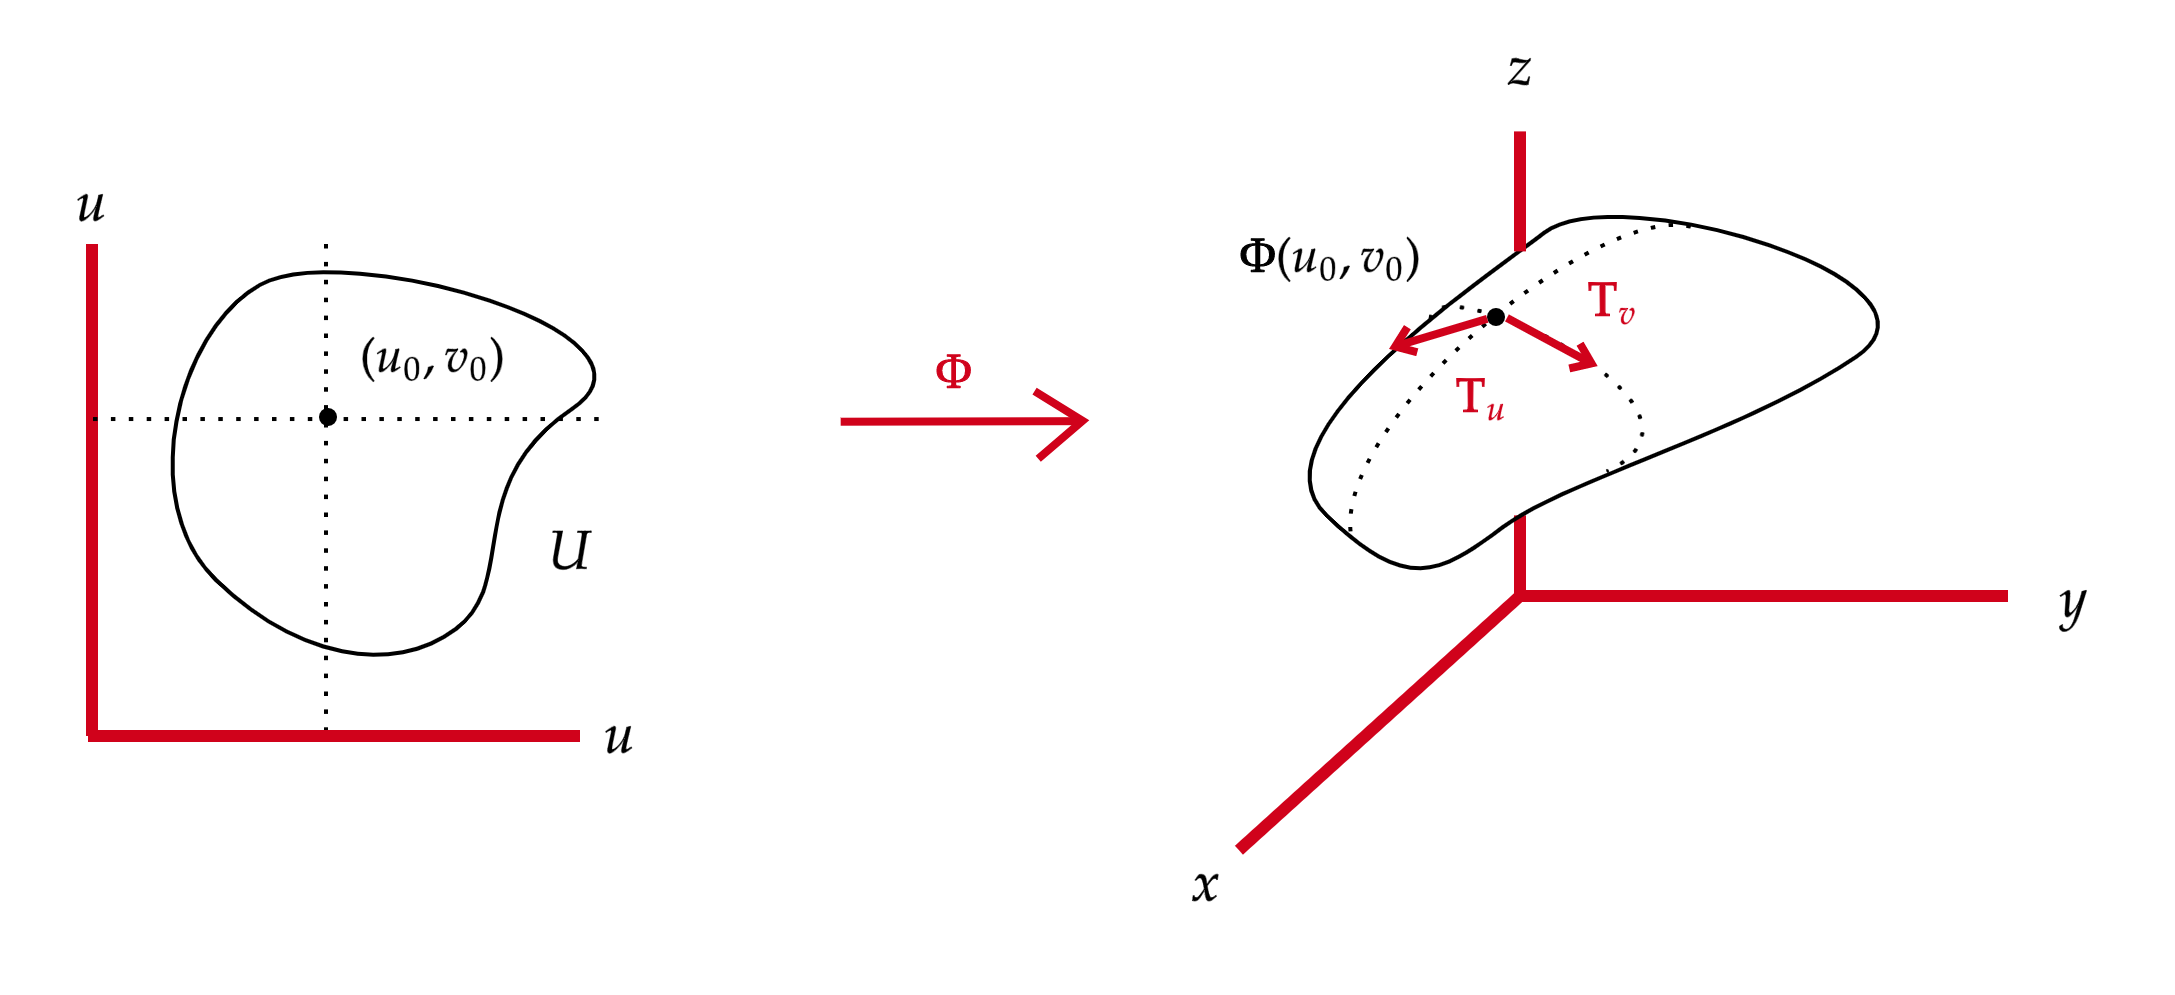
\includegraphics[width=\linewidth]{figures/wk-6/fig-13.png}
\end{center}

\hfill 

\noindent Suppose that $\mathbf{\Phi}$ is differentiable at $(u,v) \in \R^2$. The tangent vectors  $\mathbf{T}_u$ and $\mathbf{T}_v$ to the curves $\Phi(t, u_0)$ and $\Phi(t, v_0)$ on the surface are,
\begin{align*}
	&\mathbf{T}_v=\frac{\partial \boldsymbol{\Phi}}{\partial v}=\frac{\partial x}{\partial v}\left(u_0, v_0\right) \mathbf{i}+\frac{\partial y}{\partial v}\left(u_0, v_0\right) \mathbf{j}+\frac{\partial z}{\partial v}\left(u_0, v_0\right) \mathbf{k} \\
	&\mathbf{T}_u=\frac{\partial \boldsymbol{\Phi}}{\partial u}=\frac{\partial x}{\partial u}\left(u_0, v_0\right) \mathbf{i}+\frac{\partial y}{\partial u}\left(u_0, v_0\right) \mathbf{j}+\frac{\partial z}{\partial u}\left(u_0, v_0\right) \mathbf{k}
\end{align*}

\begin{rmk}
	$\mathbf{T}_u \times \mathbf{T}_v$ is normal to the surface at the point $(u_0, v_0)$.
\end{rmk}

\begin{defn}[Regular Surface]
	\sloppy We say that a surface $S$ is \textbf{regular at $\Phi(u_0, v_0)$} is $\mathbf{T}_u \times \mathbf{T}_v \neq 0$ at $(u_0, v_0)$. If this condition holds at all points on the surface, then $S$ is called \textbf{regular}.
\end{defn}

\begin{marginfigure}
	The condition that $\mathbf{T}_u \times \mathbf{T}_v(u,v) \neq 0$ suggests that the partials $\mathbf{\Phi}_u$ and $\mathbf{\Phi}_v$ are linearly independent everywhere, which ensures the existence of the tangent plane at every point of $\mathbf{\Phi} = S$.
\end{marginfigure}

\begin{ex}{$\mathbf{\Phi}(u, v)=(u, v, f(u, v))$}{label}
	Given a $C^1$ function $f$, define the map $\mathbf{\Phi}(u, v)=(u, v, f(u, v))$. We have that $\mathbf{T}_u = (1, 0, f_u)$ and $\mathbf{T}_v = (0, 1, f_v)$. Therefore,
	\[\mathbf{T}_v \times \mathbf{T}_v=\left|\begin{array}{lll}
		i & j & k \\
		1 & 0 & f_v \\
		0 & 1 & f_v
		\end{array}\right|=-f_v \cdot \mathbf{i}-f_v \cdot \mathbf{j}+ \mathbf{k} \neq \mathbf{0}\]
		regardless of our choice of $f$.
\end{ex}

\begin{ex}{Upper Sheet of a Cone}{label}
	The upper sheet of a cone is given by,
	\[\mathbf{\Phi}(u, v)=(u \cos v, u \sin v, u)\]
	where $u \geq 0$ and $0 < v < 2 \pi$. Here,
	\begin{align*}
		&\mathbf{T}_u=(\cos v, \sin v, 1) \\
		&\mathbf{T}_v=(-u \sin v, u \cos v, 0)
	\end{align*}
	and consequently,
	\[\mathbf{T}_v \times \mathbf{T}_v=\left|\begin{array}{ccc}
	i & j & k \\
	\cos v & \sin v & 1 \\
	-u \sin v & u \cos v & 0
	\end{array}\right|=-u \cos v \mathbf{i}-u \sin v \mathbf{j}+u \mathbf{k}\]
	We have that $\mathbf{T}_u \times \mathbf{T}_v = \mathbf{0}$ if and only if $\|\mathbf{T}_u \times \mathbf{T}_v\| = \mathbf{0}$ and,
	\[\left\|\mathbf{T}_u \times \mathbf{T}_v\right\|=\left(u^2 \cos ^2 v+u^2 \sin ^2 v+u^2\right)^{1 / 2} = 2 \sqrt{u}\]
	which is $\mathbf{0}$ if and only if $u = 0$.
\end{ex}

\begin{marginfigure}
    The \textbf{upper sheet of the cone} is,
    \[\mathbf{\Phi}(u, v)=(u \cos v, u \sin v, u)\]
    \begin{center}
       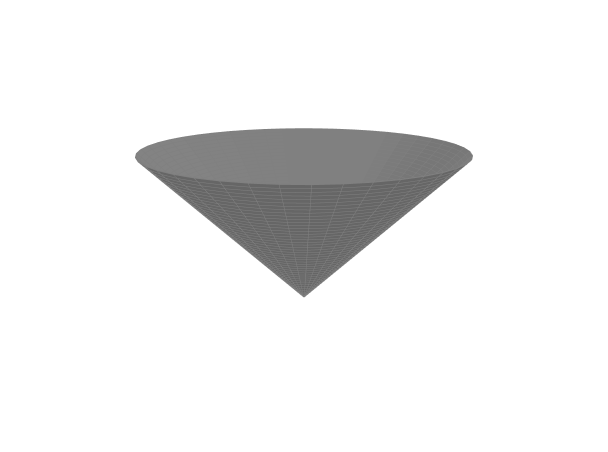
\includegraphics[width=\textwidth]{figures/wk-6/fig-14.png}
    \end{center}
    
    \LineBreak

    The \textbf{helicoid} is,
    \[\mathbf{\Phi}(u, v)=(u \cos v, u \sin v, v)\]
    \begin{center}
        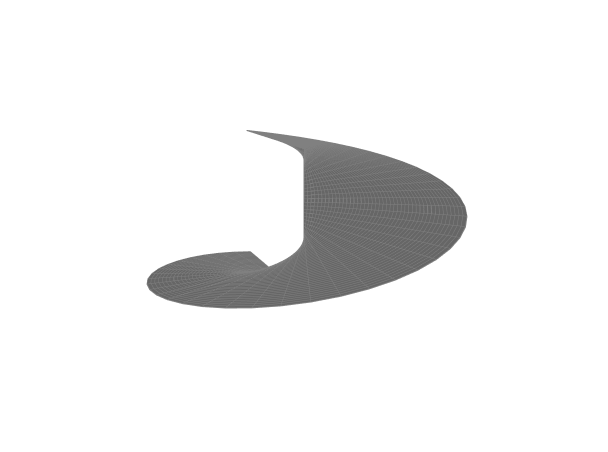
\includegraphics[width=\textwidth]{figures/wk-6/fig-15.png}
    \end{center}
    
\end{marginfigure}

\begin{ex}{Helicoid}{label}
	The helicoid is given by,
	\[\mathbf{\Phi}(u, v)=(u \cos v, u \sin v, v)\]
	where $u \geq 0$ and $0 < v < 2 \pi$. Here,
	\begin{align*}
		&\mathbf{T}_u=(\cos v, \sin v, 0) \\
		&\mathbf{T}_v=(-u \sin v, u \cos v, 1)
	\end{align*}
	and consequently,
	\[\mathbf{T}_u \times \mathbf{T}_v=\left|\begin{array}{ccc}
	i & j & k \\
	\cos v & \sin v & 0 \\
	-u \sin v & u \cos v & 1
	\end{array}\right|\]
	Observe that this is equal to,
	\[\operatorname{sinv} \mathbf{i}-\cos v \mathbf{j}+u \mathbf{k}\]
	Hence, $\left\|\mathbf{T}_u \times \mathbf{T}_v\right\|=\sqrt{1+u^2} \neq 0$ for all $u$.
\end{ex}

\hfill

\noindent In the next example, we will see how to parameterize the \textbf{torus of revolution}. This is summarized in the diagram below:

\begin{center}
   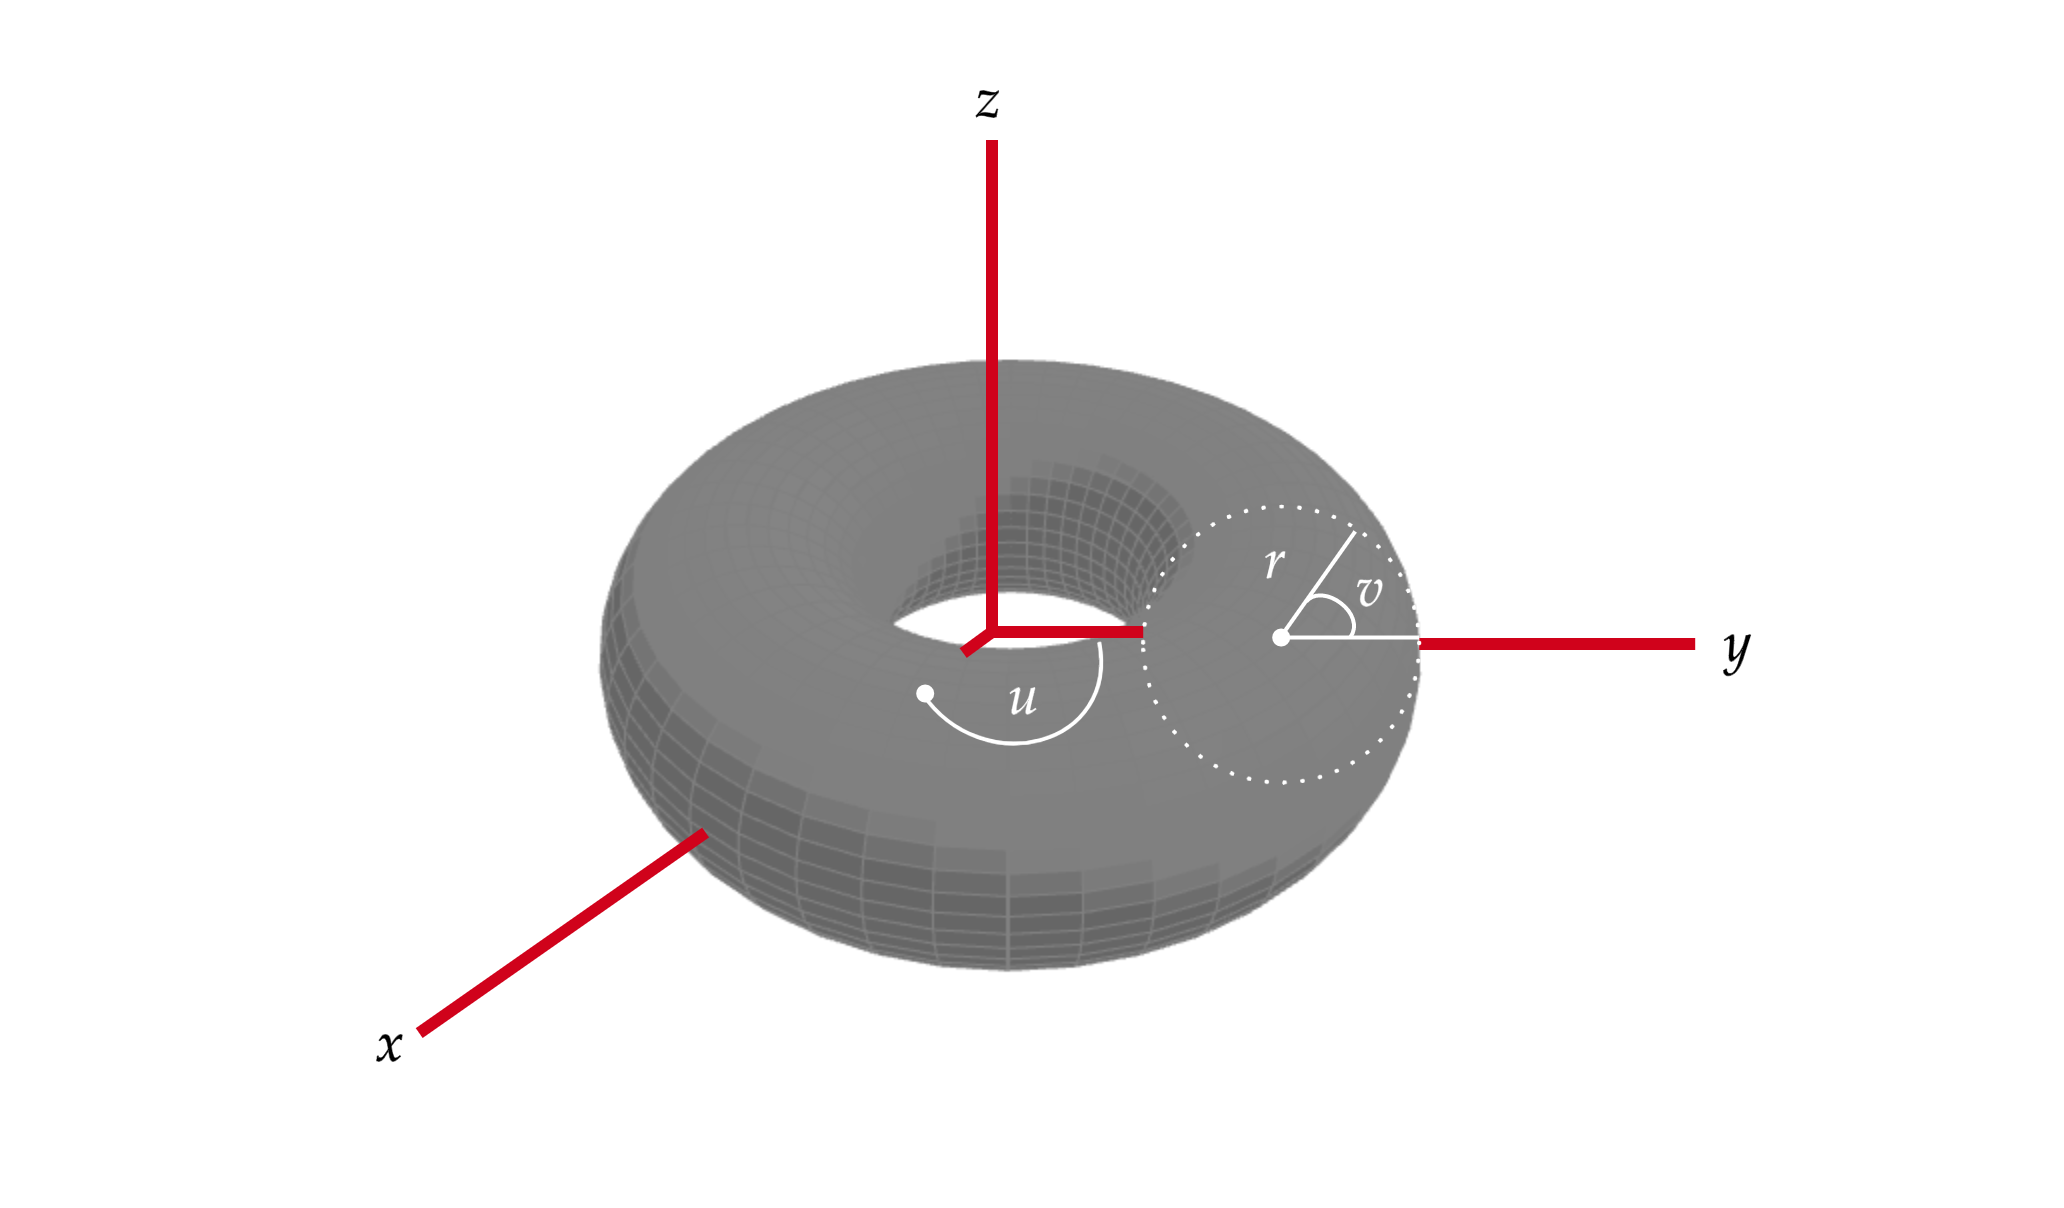
\includegraphics[width=\textwidth]{figures/wk-6/fig-16.png}
\end{center}

\begin{ex}{Torus of Revolution}{label}
	The torus of revolution $\mathbf{\Phi}(u, v)$ is given by,
	\begin{align*}
		&x(u, v)=(a+r \cos v) \cos u \\
		&y(u, v)=(a+r \cos v) \sin u \\
		&z(u, v)=r \sin v
	\end{align*}
	where $0 < u, v < 2 \pi$. Here,
	\begin{align*}
		&\mathbf{T}_u=(-\sin u(a+r \cos v), \cos u(a+r \cos v), 0) \\
		&\mathbf{T}_v=(-r \sin v \cos u,-r \sin v \sin u, r \cos v)
	\end{align*}
	Computing the cross-product and simplifying gives,
	\[\|\mathbf{T}_u \times \mathbf{T}_v\| = r|(a+r \cos v)|\]
	which is non-zero if $r \neq 0$ and $a > r$.
\end{ex}

\begin{ex}{Sphere}{label}
	Using the \textbf{spherical coordinate transformation},
	\[\mathbf{\Phi}(u, v) = (a \sin v \cos u, a \sin v \sin u, a \cos v)\]
	is a \textbf{sphere of radius $a$} where $0 < u < 2 \pi$ and $0 < v < \pi$.
	\begin{align*}
		&\mathbf{T}_u=(-a \sin v \sin u, a \sin v \cos u, 0) \\
		&\mathbf{T}_v=(a \cos v \cos u, a \cos v \sin u,-a \sin v)
	\end{align*}
	Taking the cross-product and simplifying gives,
	\[\|\mathbf{T}_u \times \mathbf{T}_v\| = a^2 \sin v\]
	which is zero if $v = 0, \pi$.
\end{ex}

\begin{rmk}
	As shown in the previous example, the condition that
	\[\|\mathbf{T}_u \times \mathbf{T}_v\| \neq \mathbf{0}\]
	is necessary but not sufficient for the existence of a tangent plane.
\end{rmk}

\subsection{Area of a Surface}
In this chapter, we will consider piecewise regular surfaces that are unions of images of parametrized surfaces $\boldsymbol{\Phi}_i: D_i \rightarrow \mathbb{R}^3$ for which:
\begin{itemize}
	\item $D_i$ is an elementary region in the plane
	\item $\Phi_i$ is $C^1$ and one-to-one, except possibly at the boundary
	\item $S_i$ is regular except possibly at a finite number of points
\end{itemize}

\begin{defn}[Surface Area]
	The \textbf{surface area} $A(S)$ is,
	\[A(S) = \iint_U\left\|\mathbf{T}_u \times \mathbf{T}_v\right\| d u d v\]
	where $S$ is a parameterized surface.
\end{defn}

\begin{marginfigure}
	If $S$ is the union of surfaces $S_i$, then the area is the sum of the areas of $S_i$.
\end{marginfigure}

\begin{marginfigure}
	To find the surface area of a function, we are scaling by the area of the parallelogram spanned by $\mathbf{T}_u$ and $\mathbf{T}_v$.
\end{marginfigure}

\begin{ex}{Area of a Sphere}{label}
	In this example, we will verify the standard formula for the \textbf{area of a sphere}. Since $\|\mathbf{T}_u \times \mathbf{T}_v\| = a^2 \sin v$,
	\begin{align*}
		A(S) &= \int_{v=0}^{v=\pi} \int_{u=0}^{u=2 \pi}\left\|\mathbf{T}_u \times \mathbf{T}_v\right\| du d v \\
		&= 2 \pi a^2 \int_0^\pi \sin v d v \\
		&= 4 \pi a^2
	\end{align*}
\end{ex}

\begin{marginfigure}
	\textbf{Exercise:} Compute the area of a cylinder of radius $a$ and height $h$.
	\[\mathbf{\Phi}(u,v) = (a \cos v, a \sin v, u)\]
	where $0 < v < 2 \pi$ and $0 < u < h$.
\end{marginfigure}

\subsection{Integrals of Scalar Functions Over Surfaces}
In this section, we will define the integral of a \textbf{scalar function} $f$ over a surface $S$. This generalizes the area of a surface, which corresponds to the integral over $S$ of the scalar function $f(x, y, z) = 1$. Consider a surface $S$ parameterized by a mapping $\mathbf{\Phi} : D \rightarrow S \subseteq \R^3$, where $D$ is an elementary region. We write,
\[\Phi(u, v)=(x(u, v), y(u, v), z(u, v))\]

\begin{defn}[Integral of a Scalar Function Over a Surface]
	Let $f: \R^3 \rightarrow \R$ be a continuous function defined on a parameterized surface $S$.
	\[\iint_S f(x, y, z) d S =\iint_S f d S=\iint_D f(\boldsymbol{\Phi}(u, v))\left\|\mathbf{T}_u \times \mathbf{T}_v\right\| d u d v\]
	is the \textbf{integral of $f$ over $S$}.
\end{defn}

\begin{marginfigure}
	The surface integral is independent of the choice of the parameterization.
\end{marginfigure}

\begin{rmk}
	We can compute the \textbf{average value} of a function $f$ as,
	\[\frac{\iint_S f ds}{|A(S)|}\]
\end{rmk}

\begin{ex}{Average over a Cone}{label}
	We want to compute the average of the surface defined by,
	\[f(x, y, z) = x + z^2\]
	where $D$ is the portion of the cone $x^2 + y^2 = z^2$ for which $1 \leq z \leq 4$. Parameterize the graph $z = f(x, y) = \sqrt{x^2 + y^2}$.
	\[\Phi(u, v)=\left(u, v, \sqrt{u^2+v^2}\right)\]
	Taking the appropriate partials $\mathbf{T}_u$ and $\mathbf{T}_v$,
	\[\mathbf{T}_u = \left(1, 0, \frac{u}{\sqrt{u^2+v^2}}\right) \quad \quad \mathbf{T}_v = \left(0, 1, \frac{v}{\sqrt{u^2+v^2}}\right)\]
	gives $\|\mathbf{T}_u \times \mathbf{T}_v\| = \sqrt{2}$. Next,
	\begin{align*}
		\iint_S f d S & =\iint_D f(\Phi(u, v))\left\|\mathbf{T}_u \times \mathbf{T}_v\right\| d u d v \\
		& =\iint_D\left(u+u^2+v^2\right) \sqrt{2} d u d v
	 \end{align*} 
	 We can use \textbf{polar coordinates} to compute this integral,
	 \[\int_{\theta=0}^{\theta=2 \pi} \int_{r=1}^{r=4}\left(r \cos \theta+r^2\right) r \sqrt{2} d r d \theta = \sqrt{2} \cdot 15 \pi\]
	 Hence, the average value of $f$ is,
	 \[\frac{\iint_S f ds}{|A(S)|} = \frac{255}{30} = 8.5\]
\end{ex}

\begin{marginfigure}
	\begin{center}
	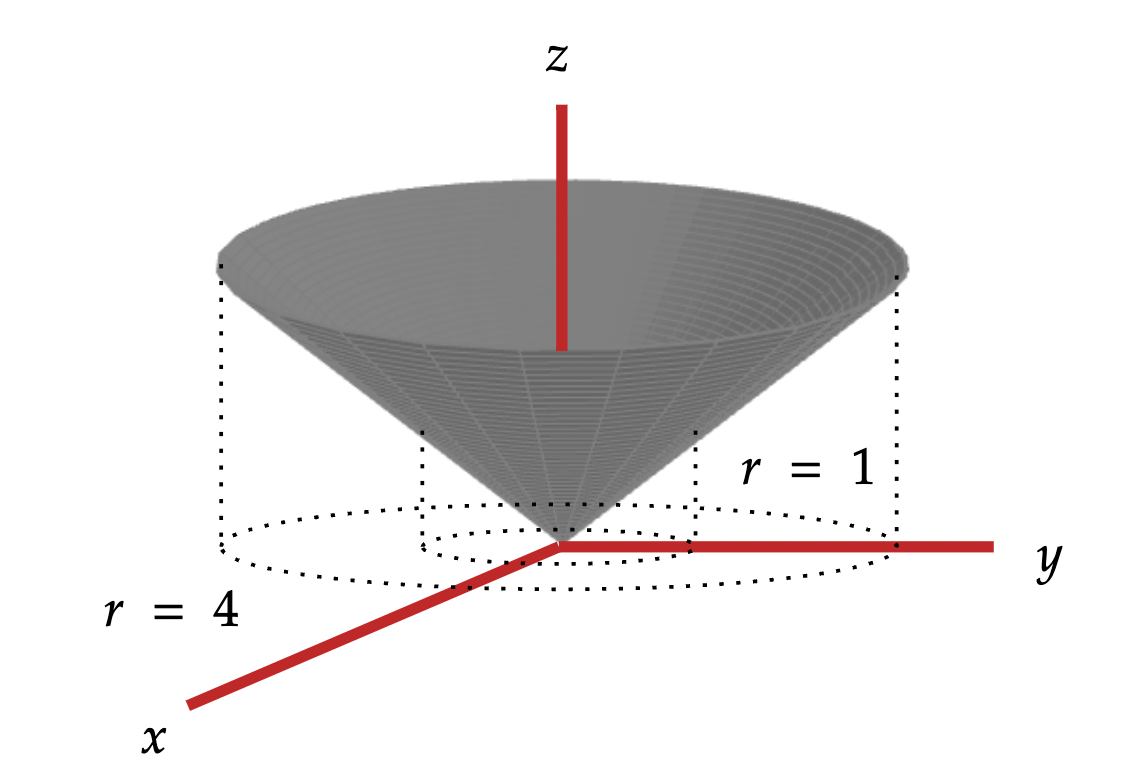
\includegraphics[width=\linewidth]{figures/wk-6/fig-18.png}
	\end{center}
\end{marginfigure}

\subsection{Oriented Surfaces}

\noindent An \textbf{oriented surface} is a two-sided surface with one side specified as positive ("outside") and one side specified as negative ("inside"). At each point $(x, y, z) \in S$, there are two unit normal vectors $\mathbf{n}_1$ and $\mathbf{n}_2$ satisfying $\mathbf{n}_1 = -\mathbf{n}_2$. Each of these normals can be associated with one side of the surface. Let $\boldsymbol{\Phi}: D \rightarrow \mathbb{R}^3$ be a parametrization of an oriented surface $S$. Suppose  that $S$ is regular at $\boldsymbol{\Phi}\left(u_0, v_0\right)$. Let $\mathbf{n}\left(\boldsymbol{\Phi}\left(u_0, v_0\right)\right)$ be the unit normal to $S$ at $\mathbf{\Phi}(u_0, v_0)$. Since,
\[\frac{\left(\mathbf{T}_{u_0} \times \mathbf{T}_{v_0}\right) }{\left\|\mathbf{T}_{u_0} \times \mathbf{T}_{v_0}\right\|}\]
\sloppy exists, it is defined and equal to $\pm \mathbf{n}\left(\Phi\left(u_0, v_0\right)\right)$.

\begin{rmk}
	$\Phi$ is called \textbf{orientation-preserving} if we have the $+$ sign, and \textbf{orientation-reversing} if we have the $-$ sign.
\end{rmk}

\begin{marginfigure}
	The definition of an oriented surface given in this section assumes that a surface has two sides. This is in fact not necessary, e.g., the Möbius strip.
\end{marginfigure}

\begin{rmk}
	Any one-to-one parameterized surface for which \text{$\mathbf{T}_v \times \mathbf{T}_u \neq 0$} can be considered as an oriented surface with a positive side determined by the direction of $\mathbf{T}_v \times \mathbf{T}_u$.
\end{rmk}

\begin{thm}
	Let $S$ be an oriented surface and let $\mathbf{\Phi}_1$ and $\mathbf{\Phi}_2$ be two regular orientation-preserving parametrizations, with $\mathbf{F}$ a continuous vector field defined on $S$. Then
	\[\iint_{\boldsymbol{\Phi}_1} \mathbf{F} \cdot d \mathbf{S}=\iint_{\boldsymbol{\Phi}_2} \mathbf{F} \cdot d \mathbf{S}\]
	If $\boldsymbol{\Phi}_1$ and $\boldsymbol{\Phi}_2$ are orientation-reversing, then
	\[\iint_{\boldsymbol{\Phi}_1} \mathbf{F} \cdot d \mathbf{S}=-\iint_{\boldsymbol{\Phi}_2} \mathbf{F} \cdot d \mathbf{S}\]
	If $f$ is a real-valued continuous function defined on $S$, and if $\boldsymbol{\Phi}_1$ and $\boldsymbol{\Phi}_2$ are parametrizations of $S$, then
	\[\iint_{\mathbf{\Phi}_1} f d S=\iint_{\mathbf{\Phi}_2} f d S\]
\end{thm}

\subsection{Surface Integrals of Vector Fields}
We can define the integral of a vector field $\mathbf{F}$ over a surface $S$.

	\begin{center}
	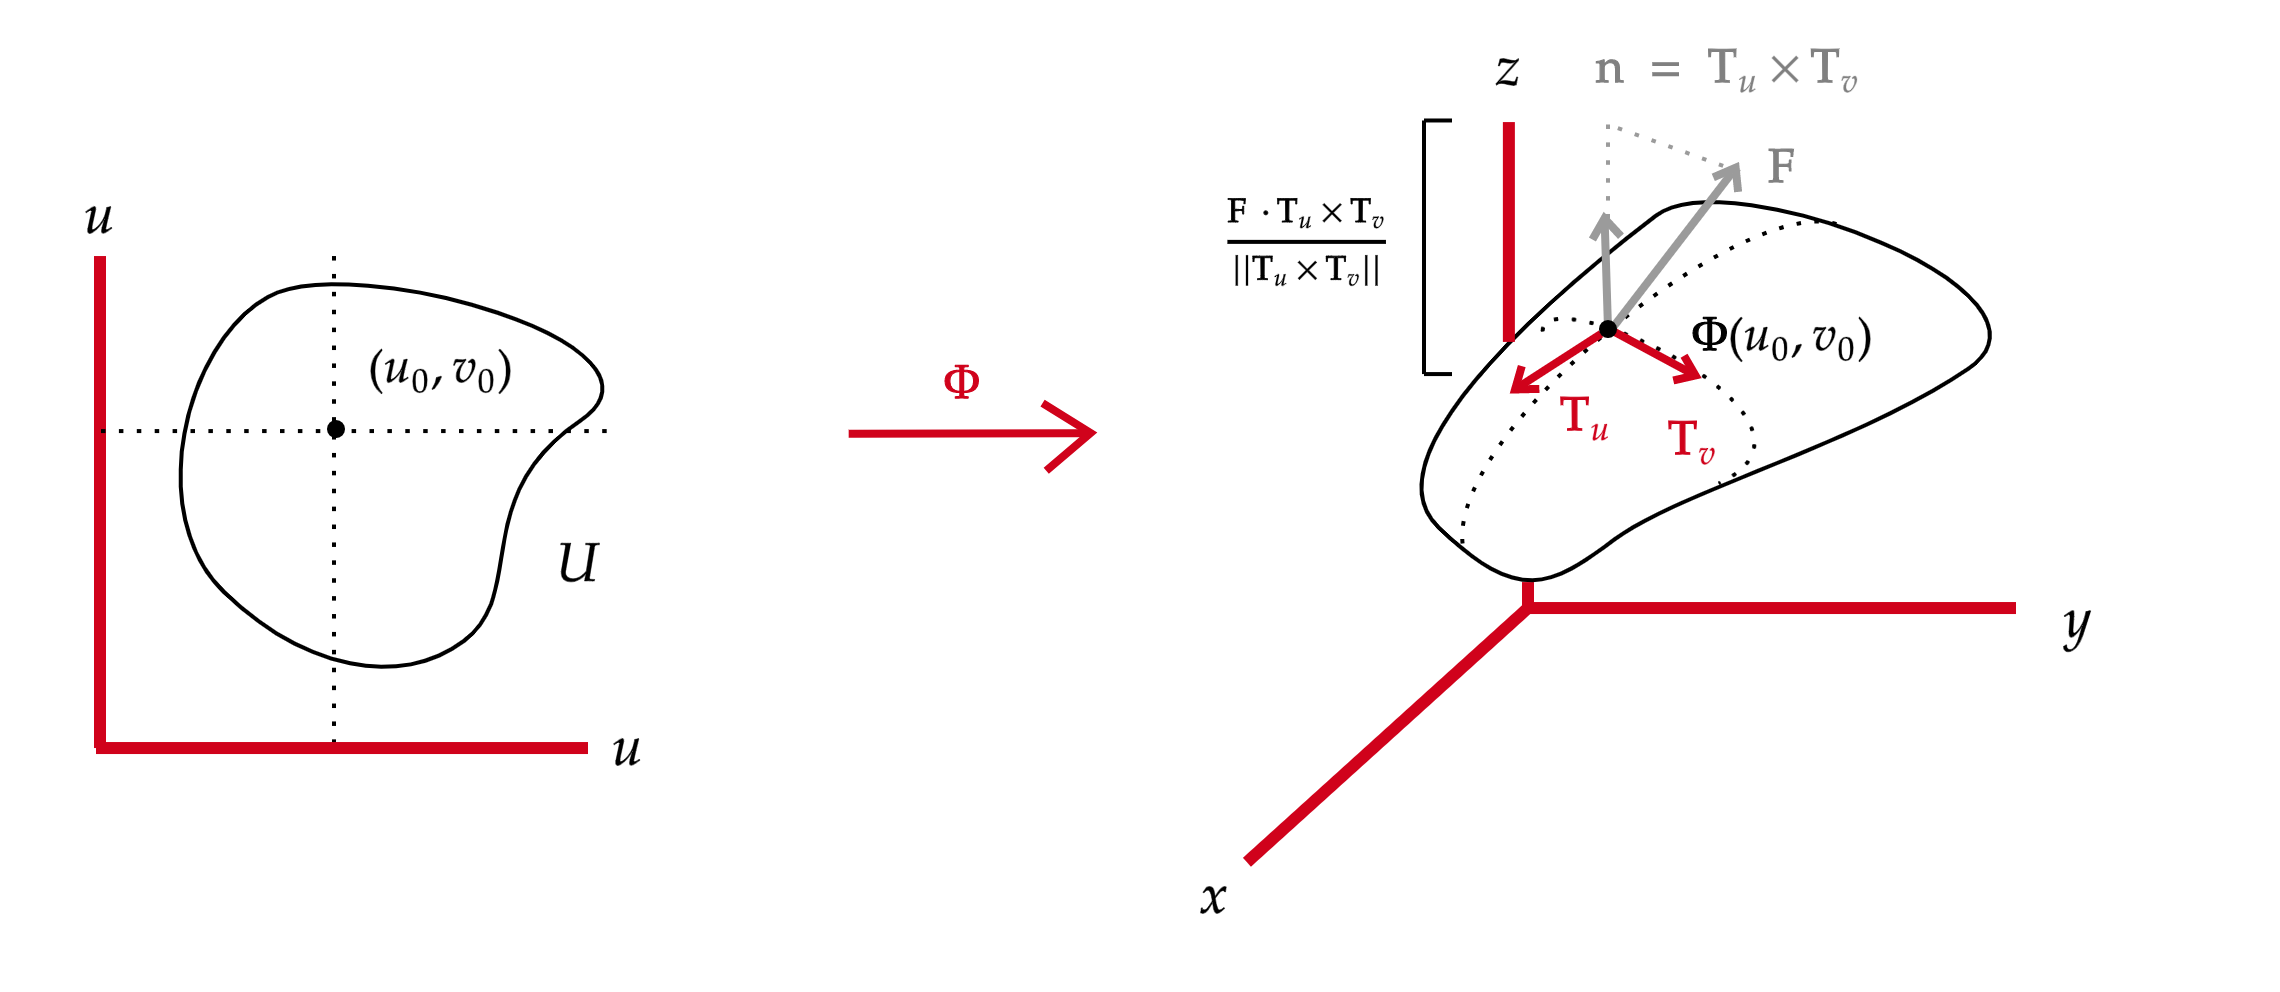
\includegraphics[width=\linewidth]{figures/wk-6/fig-19.png}
	\end{center}

\begin{defn}[Surface Integral of Vector Fields]
	\sloppy Let $\mathbf{F}$ be a vector field defined on a surface $S$, the image of a parameterized surface $\mathbf{\Phi}$.
	\[\iint_{\boldsymbol{\Phi}} \mathbf{F} \cdot d \mathbf{S}=\iint_D \mathbf{F} \cdot\left(\mathbf{T}_u \times \mathbf{T}_v\right) d u d v\]
	is the \textbf{surface integral of $F$ over $\Phi$}.
\end{defn}

\begin{rmk}
	This integral quantifies the \textbf{flux} of $\mathbf{F}$ across $S$.
\end{rmk}

\begin{rmk}
	The integral $\iint_{\boldsymbol{\Phi}} \mathbf{F} \cdot d \mathbf{S}$ is not dependent on the choice of parameterization for $S$, but it does depend on the orientation.
\end{rmk}

